\documentclass[12pt,a4paper,openany]{article}

\usepackage{lmodern}
\usepackage{xcolor}
\usepackage[utf8]{inputenc}
\usepackage[T1]{fontenc}
\usepackage[francais]{babel}
\usepackage[top=1.7cm, bottom=1.7cm, left=1.7cm, right=1.7cm]{geometry}
%\usepackage[frenchb]{babel}
\usepackage{graphicx}
%\usepackage{layout}
%\usepackage{setspace}
%\usepackage{soul}
%\usepackage{ulem}
%\usepackage{eurosym}
%\usepackage{bookman}
%\usepackage{charter}
%\usepackage{newcent}
%\usepackage{lmodern}
%\usepackage{mathpazo}
%\usepackage{mathptmx}
%\usepackage{url}
%\usepackage{verbatim}
%\usepackage{moreverb}
%\usepackage{wrapfig}
%\usepackage{amsmath}
%\usepackage{mathrsfs}
%\usepackage{asmthm}
%\usepackage{makeidx}
%\usepackage{tikz} %Vectoriel
%\usepackage{listingsutf8}
\usepackage{fancyhdr}
\usepackage{multido}
\usepackage{amssymb}


%\definecolor{gris1}{gray}{0.40}
\definecolor{gris2}{gray}{0.55}
\definecolor{gris3}{gray}{0.65}
\definecolor{gris4}{gray}{0.50}


\lstdefinelanguage{algo}{%
   morekeywords={%
    %%% couleur 1
		importer, programme, glossaire, fonction, procedure, constante, type, 
	%%% IMPORT & Co.
		si, sinon, alors, fin, tantque, debut, faire, lorsque, fin lorsque, declancher, enregistrement, tableau, retourne, retourner, =, /=, <, >, traite,exception, 
	%%% types 
		Entier, Reel, Booleen, Caractere,
	%%% types 
		entree, maj, sortie,	
	%%% types 
		et, ou, non,
	},
  sensitive=true,
  morecomment=[l]{--},
  morestring=[b]',
}

%\lstset{language=algo,
    %%% BOUCLE, TEST & Co.
%      emph={importer, programme, glossaire, fonction, procedure, constante, type},
%      emphstyle=\color{gris2},
    %%% IMPORT & Co.
%      emph={[2]si, sinon, alors, fin , tantque, debut, faire, lorsque, fin lorsque, declancher, retourner, et, ou, non,enregistrement, retourner, retourne, tableau, /=, <, =, >, traite,exception},
%      emphstyle=[2]\color{gris1},
    %%% FONCTIONS NUMERIQUES
%      emph={[3]Entier, Reel, Booleen, Caractere},
%      emphstyle=[3]\color{gris3},
    %%% FONCTIONS NUMERIQUES
%      emph={[4]entree, maj, sortie},	
%      emphstyle=[4]\color{gris4},
%}
\lstset{ % general style for listings 
   numbers=left 
	, extendedchars=\true
   , tabsize=2 
   , frame=single 
   , breaklines=true 
   , basicstyle=\ttfamily 
   , numberstyle=\tiny\ttfamily 
   , framexleftmargin=13mm 
   , xleftmargin=12mm 
   , captionpos=b 
	, language=algo
	, keywordstyle=\color{blue}
	, commentstyle=\color{green}
	, showstringspaces=false
	, extendedchars=true
	, mathescape=true
} 
 %prise en charge du langage algo

\title{Compte rendu TP1\\ Tris et complexité}
\date{Développement en C++\\ Semestre 2\\}
\author{}
\lhead{Compte rendu TP1: Tris et complexité}
\chead{}
\rhead{Valleix - de Roquemaurel (Groupe F)}

\lfoot{Université paul sabatier Toulouse III}
\cfoot{\thepage}
\rfoot{dev2}

\pagestyle{fancy}
\begin{document}
	\maketitle
	Dans ce compte rendu nous allons étudier la compléxité de différents algorithmes de tris. \\	
	Nous allons voir: 
	\begin{itemize}
		\item Le tri à bulles
		\item Le tri de Shell
		\item Le tri Pivot
		\item Le tri par selection
	\end{itemize}
	Tous ces tris utilisent des algorithmes différents, et sont donc plus ou moins rapide, c'est ce que nous allons étudier.\\ \\ \\
	TP réalisé par \textbf{Antoine de ROQUEMAUREL} et \textbf{Fabrice VALLEIX}
		\begin{figure}[!h] 
			\begin{center}	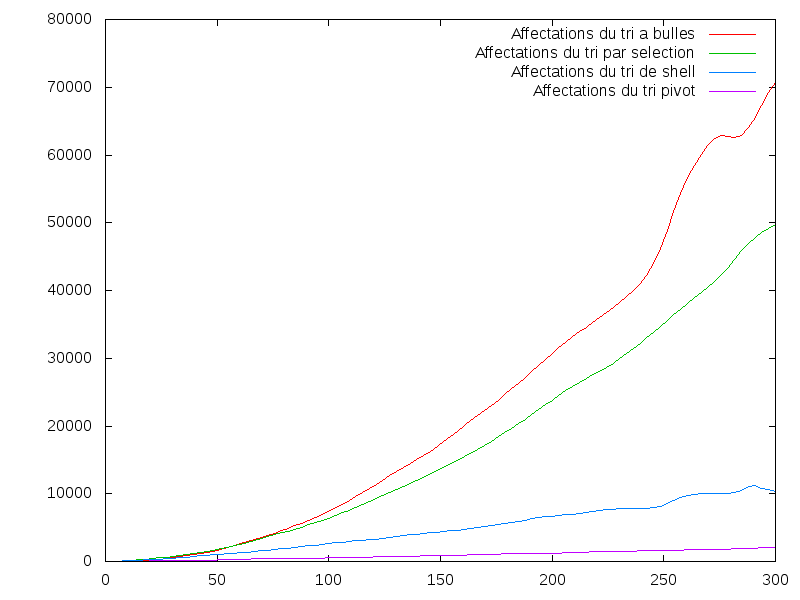
\includegraphics[height=10cm]{lesquatretris.png}										
				\caption{Les différents tris étudiés}
			\end{center}
		\end{figure}
	\newpage
	

	\section{Le tri à bulles}
		Le tri à bulle est assez lent lorsque le nombre d'élements à trier est superieur à une vingtaine. Il n'est donc pas très utilisé\\
		Sa complexité est $T(n) = O(n^{2})$
		\begin{figure}[!h] 
			\begin{center}	
				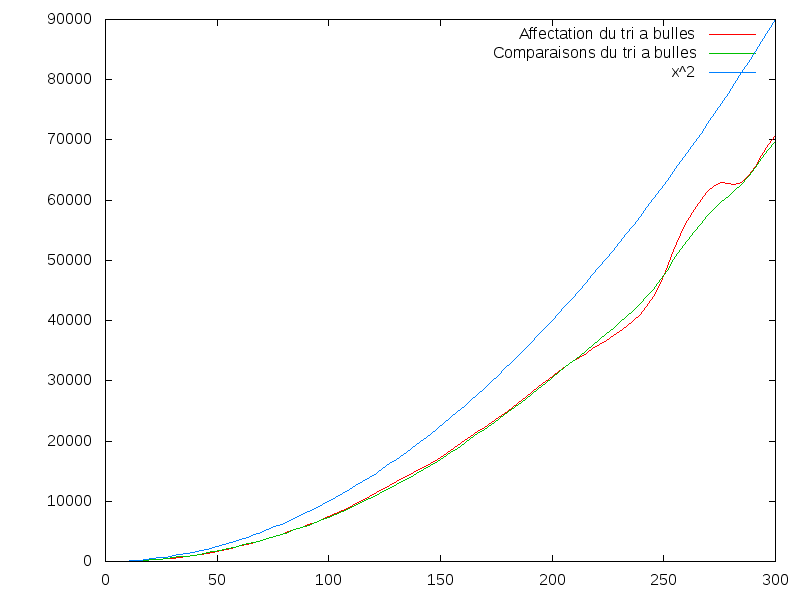
\includegraphics[height=10cm]{triBulles.png}										
				\caption{Tri à bulles}
			\end{center}
		\end{figure}
		\\ \\
			Avec l'aide de la courbe de $x^{2}$ on observe que les affectations et les comparaisons du tri à bulles sont proprotionnelles a $x^{2}$
		\newpage
	\section{Le tri de Shell}
		Le tri de Shell est une amélioration du tri par insertion. \\
		Il est beaucoup plus rapide que le tri à bulles, la compléxité du tri Shell est $T(n) = O(n\sqrt{n})$
		\begin{figure}[!h] 
			\begin{center}	
				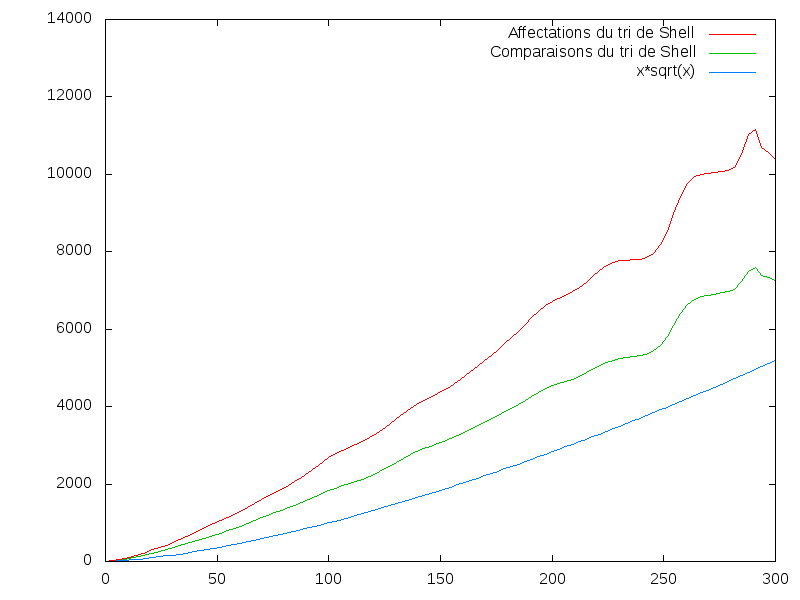
\includegraphics[height=10cm]{triShell.png}										
				\caption{Tri de Shell}
			\end{center}
		\end{figure}
		\\ \\
			Avec l'aide de la courbe de $x\sqrt{x}$ on observe que les affectations et les comparaisons du tri de shell sont proprotionnelles a $x\sqrt{x}$
		\newpage
	\section{Le tri pivot}
		Le tri pivot également appellé tri rapide est le plus rapide des tris que nous étudions. en effet sa complexité est de $T(n) = O(n\log{n})$, cependant lorsque le tableau est presque trié, il effectue autant d'affectation et de comparaisons qu'un tableau n'étant pas du tout trié, dans ce cas là il est préférable d'utiliser le tri par insertion.
		\begin{figure}[!h] 
			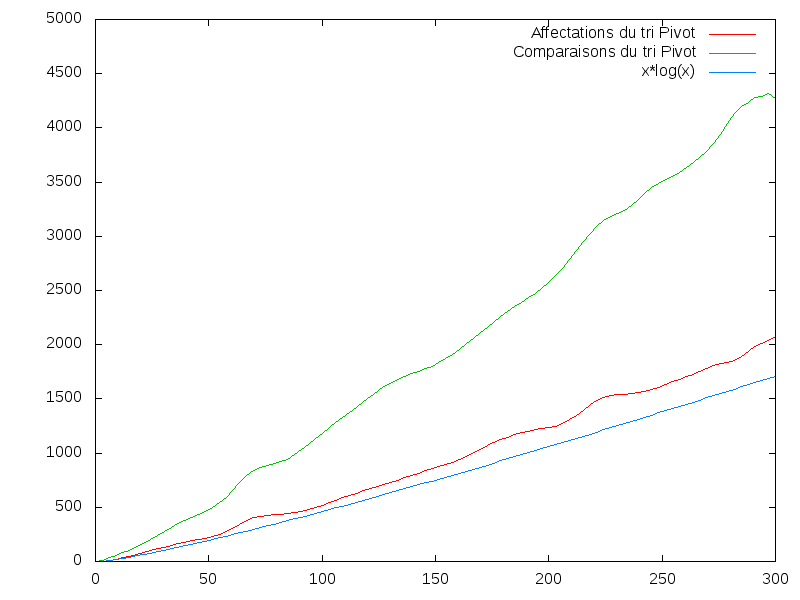
\includegraphics[height=10cm]{triPivot.png}										
			\caption{Le tri Pivot ou tri rapide}
		\end{figure}\\ \\
		On peut remarquer que les affectations du tri pivot sont proportionelle à $x\log(x)$.\\
		Cependant, le nombre de comparaisons est beaucoup plus important que le nombre d'affectations, mais le plus lent à être effectué, ce sont les affectations, cela n'est donc pas grave, et le tri pivot reste l'algorithme le plus rapide étudié dans ce compte rendu. 
		\newpage		
	\section{Le tri par séléction}
		Le tri par séléction est comme le tri à bulle un algorithme assez lent. Bien qu'il soit un petit peu plus rapide que le tri à bulle, sa complexité est la même: $T(n) = O(n\sqrt{n})$. \\
		Il peut être utilisé lorsqu'il s'agit de petit tableau à trier, dans le cas contraire, on préferera utiliser le tri pivot.
		\begin{figure}[!h] 
			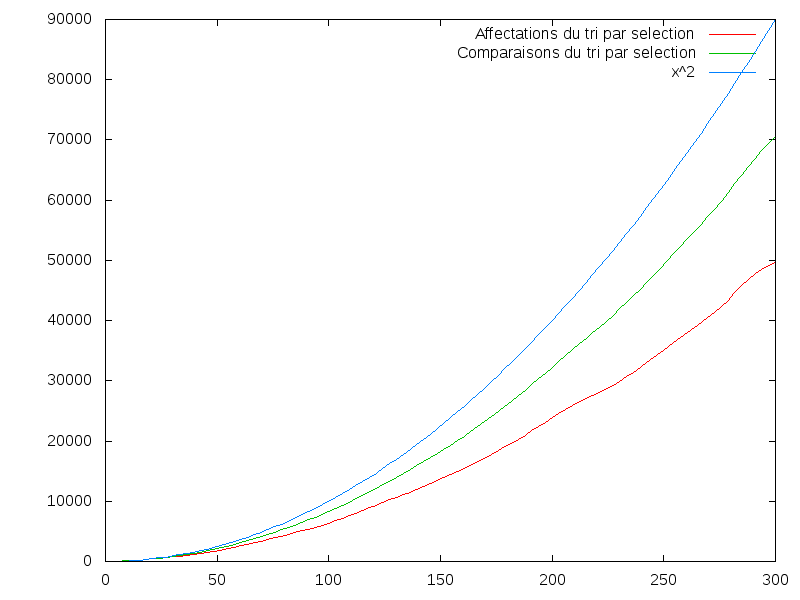
\includegraphics[height=10cm]{triSelection.png}										
			\caption{Le tri par selection}
		\end{figure}\\ \\
		Le tri par selection est donc proportionelle à $x^{2}$.
	
		\newpage
	\section{Comparaisons des tris}
		\begin{figure}[!h] 
			\begin{center}	
				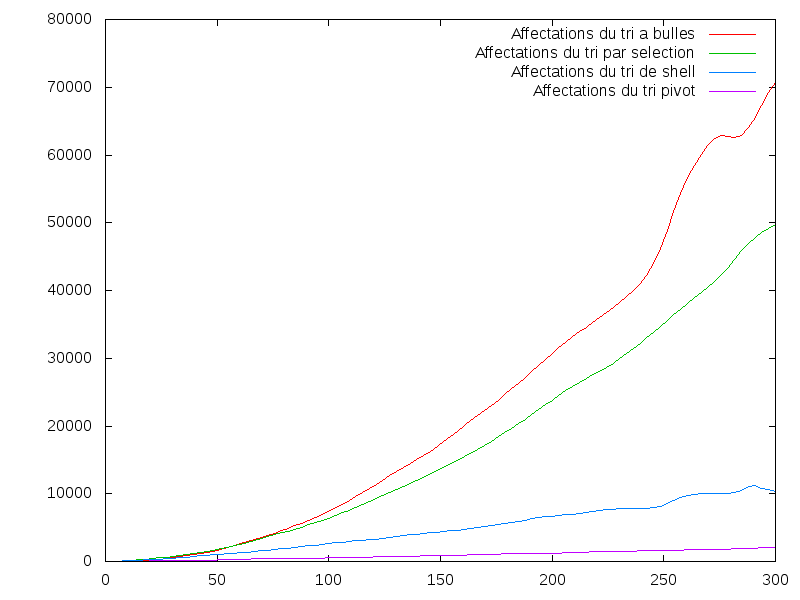
\includegraphics[height=10cm]{lesquatretris.png}										
				\caption{Comparaison des différents tris}
			\end{center}
		\end{figure}
		La courbe 6 nous montre qu'il y a deux types d'algorithmes: des algorithmes plus lent (tri à bulles et tri par selection) et d'autres plus rapide (tri de Shell et tri pivot). \\
		Ces dernier sont rapide pour des tableaux avec beaucoup d'éléments, cependant pour de petits tableaux il est préférable d'utiliser le tri à bulle ou le tri par selection, en effet ces algorithmes sont plus simple à mettre en 
		place. La différence de vitesse s'accroit de plus en plus en fonction de la taille du tableau, cela est dût au différentes complexité. \\
		Il n'existe donc pas de mauvais algorithme, il faut s'adapter et choisir un algorithme de tri en fonction de la situation.
\end{document}
